\chapter{関連研究}

\section{動機づけ}
動機づけとは,行動に駆り立て目標に向かわせる内部過程である.
デシらが提唱した自己決定論~\cite{ryan2000self}では,動機づけをその自己決定度合いに基づいて分類している.
自己決定性とは,その行動に対して見出している価値,つまり動機づけの要因が,どれほど内在的かを示す度合いである.
自己決定論における動機づけの分類は表~\ref{tb:motivation}の6種類であり,種類ごとの特徴や動機づけが生じる要因を定義している.

\begin{table}[htb]
\begin{center}
  \begin{tabular}{|l|l|} \hline
    動機づけ & 要因 \\ \hline
    非動機づけ & なし \\
    外的調整による動機づけ & 報酬や罰のため \\
    取り入れ的調整による動機づけ & 競争のため \\ 
    同一化的調整による動機づけ & 目標のため \\ 
    統合的調整による動機づけ & 習慣から \\ 
	内発的動機づけ & 好奇心から \\ \hline
  \end{tabular}
  \caption{動機づけタイプとその要因}
  \label{tb:motivation}
\end{center}
\end{table}

非動機づけは,活動に全く動機づけられていない状態である.
外的調整は,物的報酬の獲得や罰の回避を目的とする動機づけであり,これらが消滅すると同時に動機付けも減少する.
取り入れ的調整は,不安や恥ずかしさ,名誉心などから生じるものであり,自己価値を守ることが行動の目的となる.
したがって,外的要素が要因ではあるものの,価値を一部内在化できている.
同一化的調整は,行動の目的が自身の目標や目的のためとなる,行動の価値と自己が同一化できているため,自律的に行動する.
統合的調整は,習慣によるものである.
その行動が当たり前のものとなり,自己内で葛藤を生じずに活動に取り組む動機づけである.
内発的動機づけは,好奇心や関心から生じる動機づけであり,行動そのものに価値を見出している.

\begin{figure}[ht]
	\begin{center}
	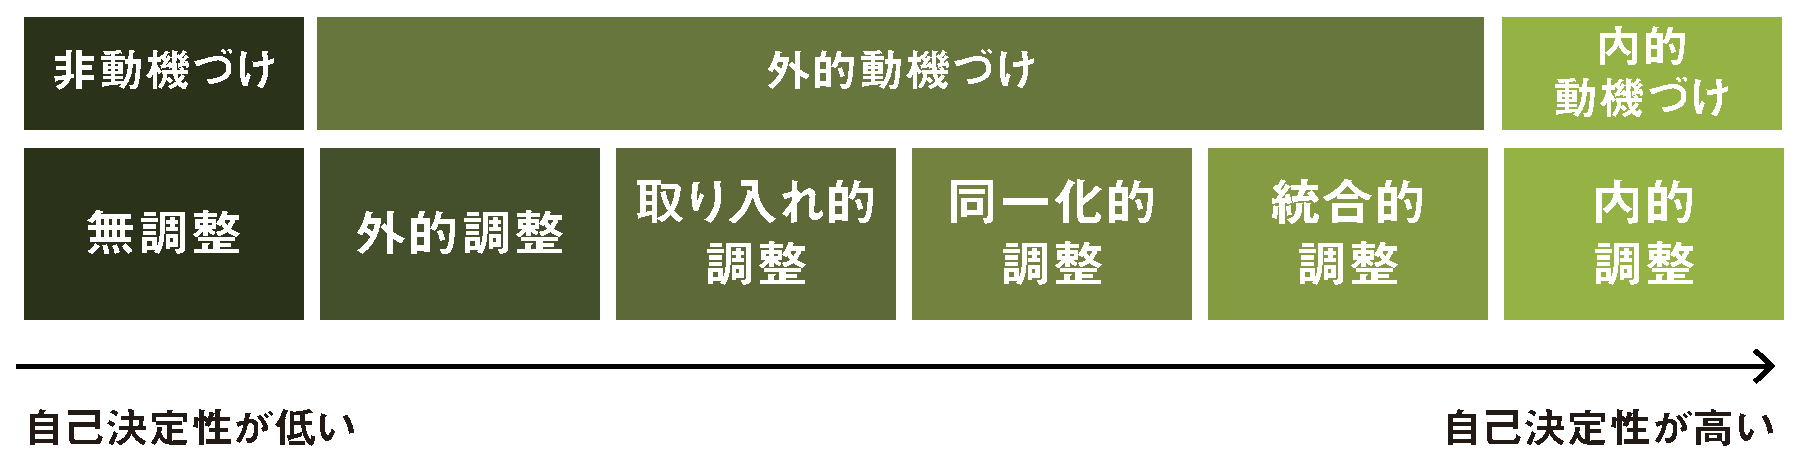
\includegraphics[width=12cm]{images/2/motivation.eps}
	\caption{動機づけタイプと自己決定性の高さ}
	\label{fig:motivation}
	\end{center}
\end{figure}

これらの動機づけタイプは,図~\ref{fig:motivation}のように自己決定性が低い順に並んでいる.
自己決定性が高いほど,つまり行動に期待する価値の所在が内的であるほど満足感が高く,より持続するとされている.
したがって,本研究の背景である``学習に対するストレス"を軽減させるには,内的な動機づけを目指すことが重要だと言える.

\section{コンピューティングによる動機づけの向上}
心理学の分野において長年研究されてきた動機づけだが,近年ではそれらの手法をコンピューティング技術によって堅牢に実現しようとする研究が多くなされている.
本節では,コンピューティングによる動機づけの向上を図った関連研究を整理する.

Johnsenら~\cite{johnsen2014mixed}は,子供の肥満解消のためのビデオゲームである``Virtual Pets"を開発した.
プレイ中の様子が図~\ref{fig:VirtualPets}である.
%このシステムでは,ユーザのワークアウトによって
ペットの肥満を解消し,技を
習得させることができる.
ペットの成長によって外的調整による動機づけを刺激することができ,子供らの運動を促した.

\begin{figure}[ht]
	\begin{center}
	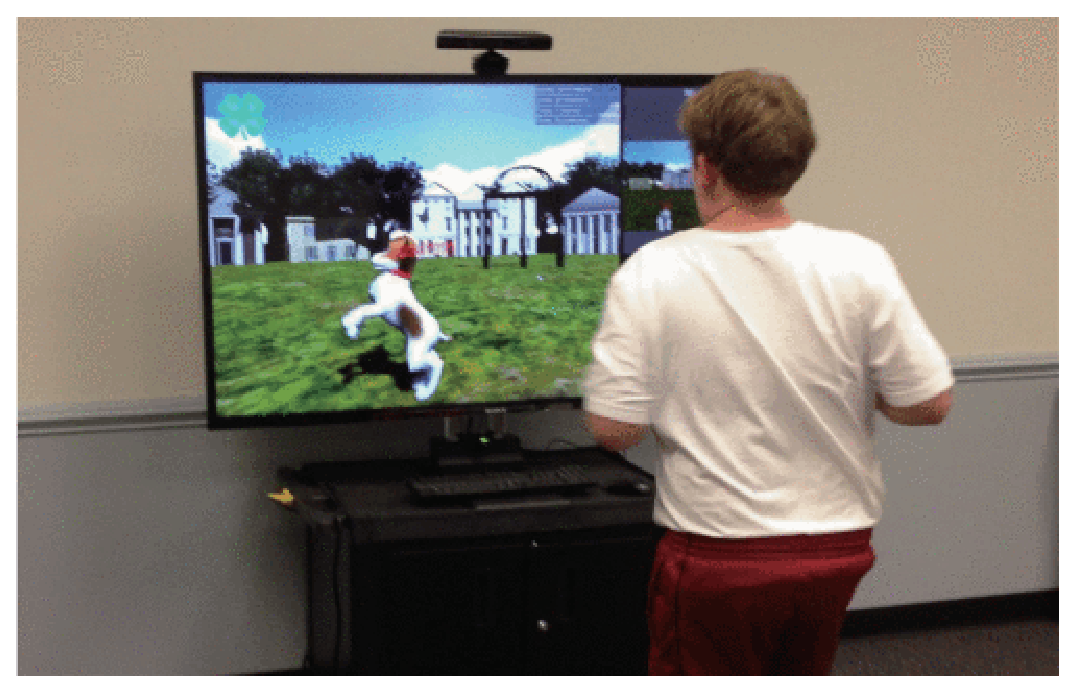
\includegraphics[width=12cm]{images/2/VirtualPets.eps}
	\caption{Virtual Pets}
	\label{fig:VirtualPets}
	\end{center}
\end{figure}

同じく運動に対する動機づけを向上させるシステムとして,Linら~\cite{lin2006fish}は``Fish’n Steps"を開発した.
これはユーザの歩数によって水槽内の魚の
成長や活動が変化するコンピュータ
ゲームである.
実際のゲーム内の画面が図~\ref{fig:fish}である.
このシステムは運動を促しただけでなく,被験者の身体活動に対する態度も向上させた.

\begin{figure}[ht]
\begin{center}
\begin{tabular}{c}
  	\begin{minipage}[b]{0.5\linewidth}
	\begin{center}
		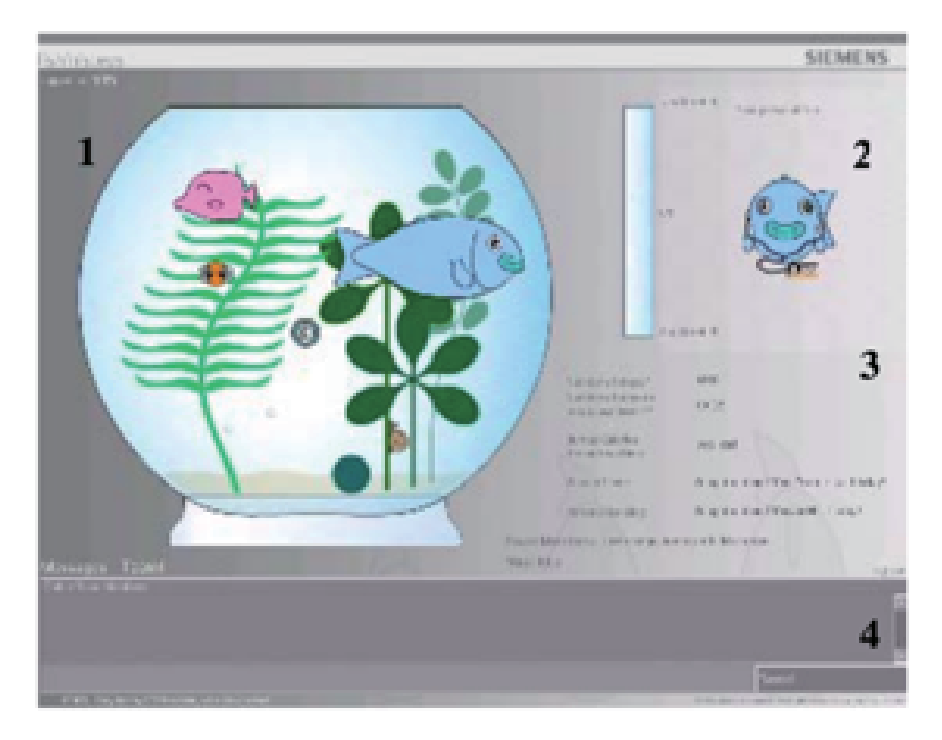
\includegraphics[width=8cm]{images/2/fish.eps}
		\caption{Fish’n Steps}
		\label{fig:fish}
	\end{center}
  	\end{minipage}

  	\begin{minipage}[b]{0.5\linewidth}
	\begin{center}
		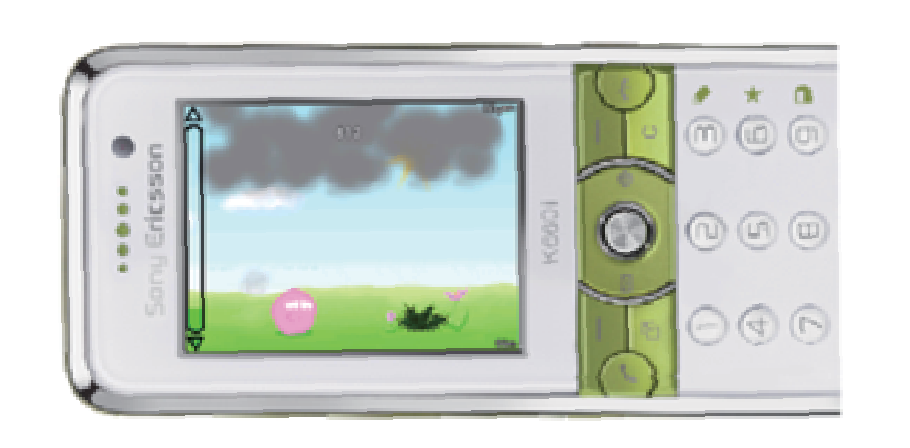
\includegraphics[width=8cm]{images/2/power.eps}
		\caption{Power explorer}
		\label{fig:power}
	\end{center}
  	\end{minipage}

\end{tabular}
\end{center}
\end{figure}

また,Gustafssonら~\cite{gustafsson2009power}が開発した``Power explorer"は,省エネルギー行動を促すモバイルゲームである.
このシステム内では,ユーザのエネルギー消費に応じて空間の
気候が変動し、モンスターの健康状態が
変化する.
実際のゲーム内の画面が図~\ref{fig:power}である.
Gustafssonらが行った評価実験では,ゲーム使用後も省エネルギー行動に対する動機づけに永続的な効果の前兆が見られた.

学習分野においても,コンピューティングを用いた動機づけ向上を図った研究が行われている.
Animal companions~\cite{Chen}はChenらが開発した``賢くない仮想キャラクタ"である.
同論文内で提案されたMy-Pet v2 systemは,このAnimal companionsを搭載した言語学習用のコンピュータゲームである.
システム内での言語学習によってAnimal companionsが成長するもので,外的調整を刺激するミニゲームや,取り入れ的調整を刺激する他者との競争などが取り入れられている.
このシステムの利用が被験者の学習意欲を高めた.

\begin{figure}[hb]
	\begin{center}
	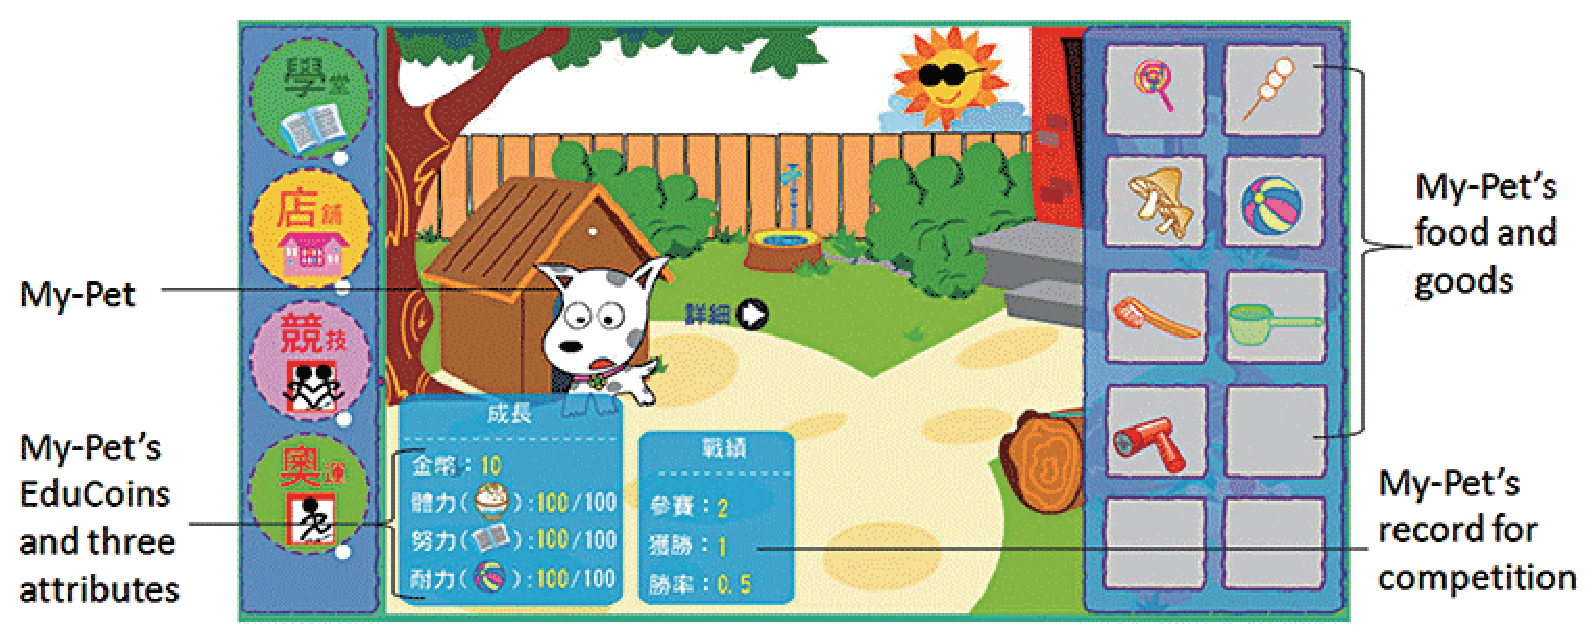
\includegraphics[width=15cm]{images/2/AnimalCompanions.eps}
	\caption{My-Pet v2 systemに搭載されたAnimal companions}
	\label{fig:animal_companions}
	\end{center}
\end{figure}

Huizengaら~\cite{huizenga2009mobile}は,Waag Societyによって開発されたThe Frequency 1550 gameを用いて,ゲームベース学習の有用性について調査した.
このモバイルゲームは,プレイを通して中世アムステルダムの歴史的知識を取得できるようになっており,ポイント獲得による外的調整へのアプローチや,競争による取り入れ的調整へのアプローチ要素が含まれている.
実際のプレイ画面は図~\ref{fig:game}である.
The Frequency 1550 gameを用いて学習した生徒と従来の授業を受けた生徒を比較すると,ゲームをプレイした生徒の方が積極的に学習に参加し,中世アムステルダムに関する知識をより多く取得することがわかった.

大即ら~\cite{otsuki}は,図~\ref{fig:hakuban}のような電子白板を用いたグループ間競争型学習支援ソフトウェアを作成した.
対話型電子白板上の教育ソフトウェアのための従来の設計指針に加え,クラスの性質に合わせた要素の調整,誤答を含めた全解答の表示を取り入れた.
このシステムには,取り入れ的調整を刺激するような競争的要素が含まれている.
2つの小学校の授業内でこのシステムを試用し,生徒らの学習意欲向上を示した.


\begin{figure}[ht]
\begin{center}
\begin{tabular}{c}
  	\begin{minipage}[b]{0.5\linewidth}
	\begin{center}
		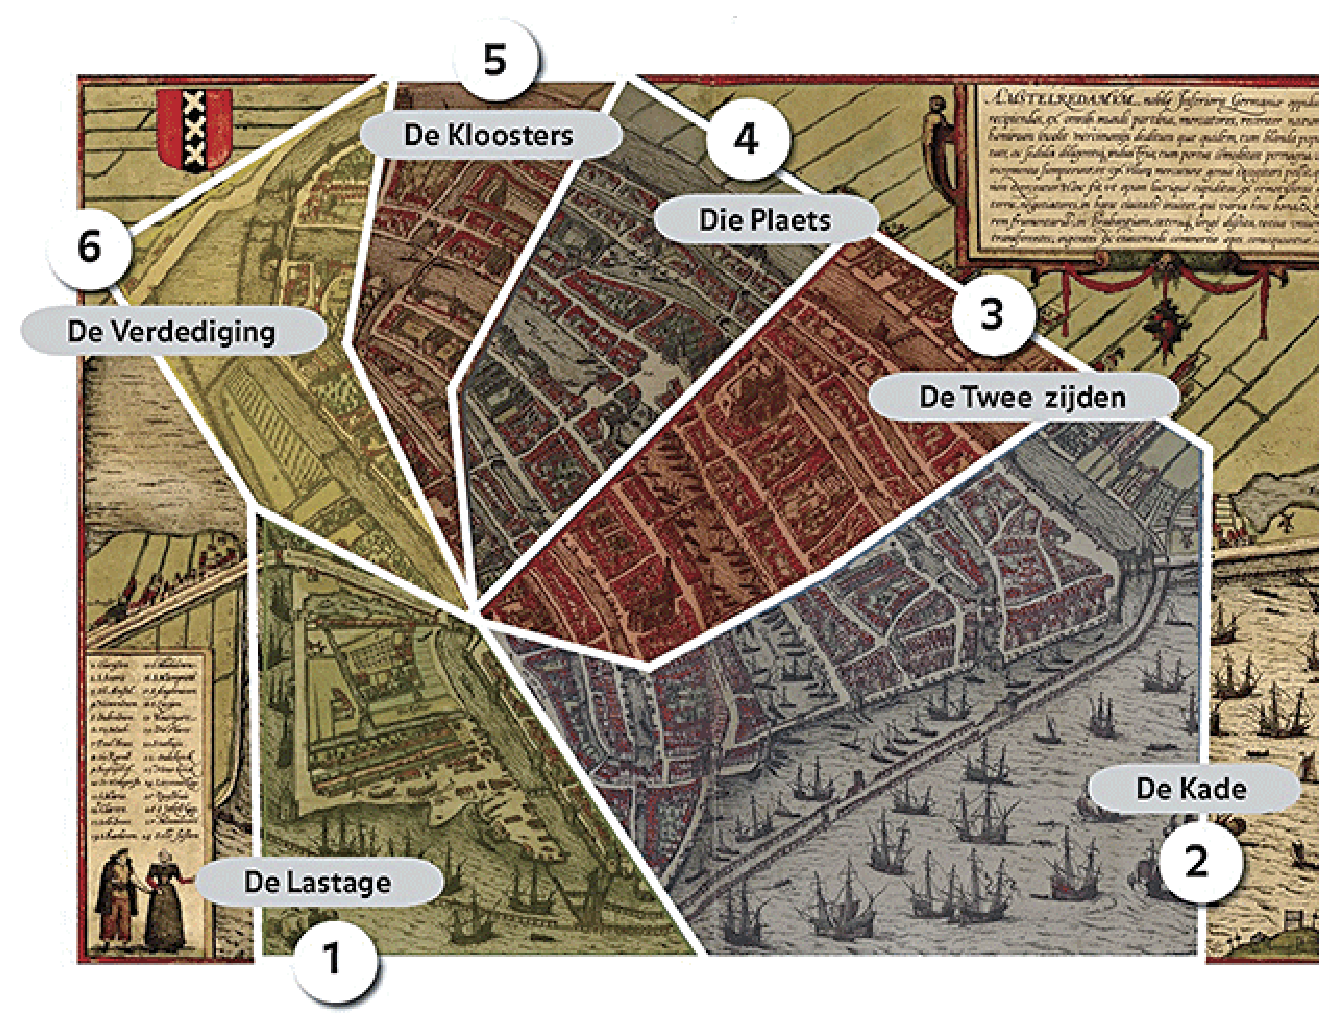
\includegraphics[width=7cm]{images/2/game.eps}
		\caption{The Frequency 1550 game}
		\label{fig:game}
	\end{center}
  	\end{minipage}

  	\begin{minipage}[b]{0.5\linewidth}
	\begin{center}
		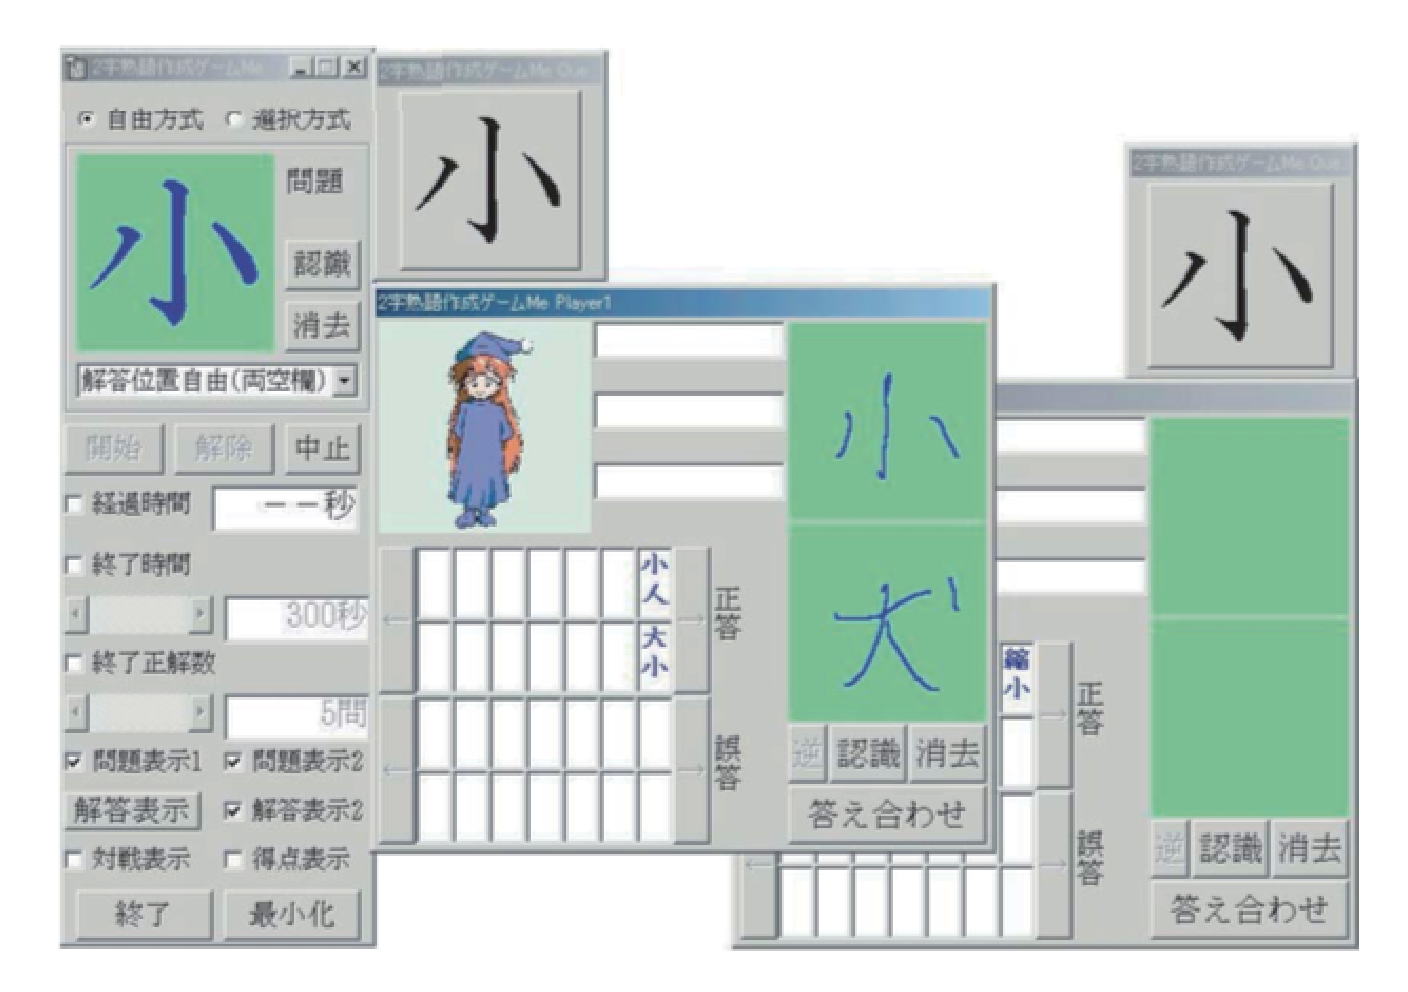
\includegraphics[width=8cm]{images/2/hakuban.eps}
		\caption{電子白板向けグループ間競争型学習支援ソフトウェア}
		\label{fig:hakuban}
	\end{center}
  	\end{minipage}

\end{tabular}
\end{center}
\end{figure}

\section{まとめ}
本章では,学習における動機づけについての関連研究を整理し,問題意識を洗い出した.
次章では,筆者が本研究に先立ち行った研究について述べ,問題意識を洗い出す.